\section{Einführung}
\label{sec:org7ca50ad}
Dieser Bericht soll eine Übersicht über den Energie- sowie den
Umweltverbrauch der Maschinenindustrie geben. Zusätzlich werden
noch die Massnahmen der Branche zum Schutz der Umwelt aufgezeigt.

\section{Umweltverbrauch der Maschinenindustrie}
\label{sec:org50f831e}
\subsection{Energieverbrauch in der Schweiz}
\label{sec:org885fcfa}

\begin{center}
\begin{tabular}{lllr}
Ressource & Menge & Prozentualer Anteil & Jahr\\
\hline
Strom \& Gas & 1595 GWh & 6.27\% & 2015\\
Öl, Kohle, etc & 3235 GWh & 12.73\% & 2015\\
Zusammen & 4'830 GWh \cite{ref7} & 19\% \cite{ref1} & 2014\\
\hline
Gesamte Schweiz & 25'421 GWh & 100\% & 2014\\
\end{tabular}

\end{center}

Diese Tabelle zeigt den Energieverbrauch der schweizer Maschinenindustrie
im Vergleich zu der restlichen Schweiz. Insgesamt geht
ca. \(\frac{1}{5}\) des gesamten Energieverbrauches zu Lasten der Industrie.
Strom und Gas Werte wurden vom Autoren grob mit Zahlen der Firma Güdel
hochgerechnet \cite{ref8}.
\newpage
\subsection{Genereller Ressourcenverbrauch}
\label{sec:orgacab74d}

\textbf{Grobe Bewertung des Rohstoffverbrauchs}
\begin{center}
\begin{tabular}{ll}
Material & Menge\\
\hline
Holz & Mittel\\
Eisen \& Stahl & Hoch\\
Aluminium & Mittel\\
Kupfer & Wenig\\
Kunststoff & Wenig\\
Chemikalien & Mittel\\
\end{tabular}

\end{center}

Holz und Aluminium werden wahrscheinlich eher in mittleren Mengen
verwendet.  Da Holz für einen effektiven Einsatz im Maschinenbau zu
schwach ist wird es oftmals nur für Verpackungen oder in
Testumgebungen eingesetzt. Aluminium ist meist zu teuer um im grossen
Stil eingesetzt zu werden. Bei grösseren Anlagen sind meist nur die
Greifer aus Aluminium um Gewicht zu sparen.

Auch Chemikalien werden wahrscheinlich im Vergleich mit den restlichen
Materialien eher in mittleren Mengen eingesetzt. Da sie oft nicht
grössere Mengen auf einmal benötigt werden.  Allerdings werden sie
nahezu in jedem Produktionsschritt eingesetzt. Etwa als Kühlmittel,
Farben und Lacke, Putzmittel oder Klebstoffe.

Kupfer kommt hauptsächlich nur in Kabeln vor und wird dadurch relativ
wenig eingesetzt. Auch Kunststoffe kommt in der Maschinenindustrie
eher weniger zum Einsatz da sie entweder den Belastungen nicht
standhalten oder wenn doch, dann oft zu teuer sind. Meistens
werden nur Verkleidungen oder ganz spezialisierte Teile aus Kunststoff
hergestellt.

Stahl ist der Werkstoff der mit Abstand am häufigsten verbaut wird da
er günstig erwerbbar ist, sehr viellseitig genutzt werden kann und dabei
auch noch sehr stabil ist.

\section{Umweltbelastung der Maschinenindustrie}
\label{sec:org0cab5a7}
\subsection{Umweltbelastung der Schweizer Maschinenindustrie}
\label{sec:orgc2f69bd}
\subsubsection{CO2 Ausstoss (2013)}
\label{sec:org9e7c3fd}
\begin{center}
\begin{tabular}{lll}
Verursacher & Menge & Prozentualer Anteil\\
\hline
Swissmem Branchen & 6.048 & 14\% \cite{ref1}\\
gesamte Industrie & 8.68 \cite{ref6} & 20.09\%\\
restliche Schweiz & 37.152 & 86\% \cite{ref1}\\
\hline
Gesamte Schweiz & 43.20 Mio. Tonnen \cite{ref6} & 100\%\\
\end{tabular}

\end{center}

Die Prozent Angaben stammen vom Swissmem und die Gesamtmengen der
Schweiz sowie der Industrie vom BAFU. Die restlichen Mengen und
Prozentangaben wurden vom Autor ergänzt.

\subsubsection{Chemische Abfälle (2016)}
\label{sec:org2becb56}

\begin{center}
\begin{tabular}{ll}
Beschreibung & Menge\\
\hline
Basen & 16533 kg\\
Farb- und Lackabfälle & 397600 kg\\
Bearbeitungsemulsionen & 39520000 l\\
Div. Maschinen- und Schmieröle & 533333 l\\
Andere Lösungsmittel & 224000 kg\\
Aufsaug- und Filtermaterial & 246133 kg\\
\end{tabular}

\end{center}

Alle Zahlen basieren auf der Entsorgungsbescheinigung \cite{ref10} der
Firma Altola welche für die Firma Güdel ausgestellt wurde. Die Zahlen
wurden jedoch vom Autoren hochgerechnet um zu versuchen den
branchenweiten Verbrauch in der Schweiz abzubilden. Dies ist jedoch
sehr inakkurat und kann allenfalls als grober Richtwert verwendet werden.

\subsection{Globaler Vergleich}
\label{sec:orgc35480b}
Ein globaler Vergleich lässt sich mangels verlässlicher Quellen nur
sehr ungenau abschätzen. Da die Schweiz auch beim Umweltschutz sehr
hohe Standards hat kann man davon ausgehen das die schweizer Industrie
nicht allzu schlecht da steht. Allerdings verursacht die schweizer
Industrie auch den grössten Anteil ihrer Umweltverschmutzung im
Ausland da die Ressourcen oftmals im Ausland hergestellt oder abgebaut
werden. Im globalen Vergleich kann wohl davon ausgegangen werden das
die Maschinenindustrie etwa so bei 20 - 30\% des gesamten CO2
Ausstosses liegt.  Zumindest lässt sich das erahnen wenn man die Werte
von China \cite{ref12} und den USA \cite{ref11} vergleicht.
\newpage
\section{Massnahmen zum Schutz der Umwelt}
\label{sec:org251d92e}
\subsection{Massnahmen der Branche}
\label{sec:orgafcd1eb}
Der Swissmem ist vor allem dafür das die einzelnen Firmen eigenständig
entscheiden können wie sie den Umweltschutz handhaben möchten.  Es
soll vor allem ein für die Forschung und Entwicklung förderliches
Umfeld geschaffen werden. Dies solle sicherstellen das aktuelle
Technologien effizienter werden. Zusätzlich sollen wirtschaftliche
Anreize geschaffen werden anstatt stattlicher Regulationen
\cite{ref5}.

Des weiteren sind sie dafür das die Schweiz ihre
Klimapolitik international angleicht damit keine zu strengen
Verordnungen die Wettbewerbsfähigkeit beinträchtigen
\cite{ref4}. Nichtsdestotrotz anerkennen sie, dass Umweltschutz
sinnvoll und wichtig ist. Allerdings sollte Umweltschutz nicht auf die
Kosten der Wirtschaftlichkeit gehen. Der Swissmem orientiert
sich dabei an der Brundtland-Definition von Nachhaltigkeit:
''Dauerhafte Entwicklung ist Entwicklung, die die Bedürfnisse der
Gegenwart befriedigt, ohne zu riskieren, dass künftige Generationen
ihre eigenen Bedürfnisse nicht befriedigen können.`` \cite{ref5}

Insgesamt sehen sie sich als wichtigen Teil bei der Verbesserung des
Umweltschutzes da die Firmen des Swissmem die eigentlichen
Technologien liefern welche dabei helfen können Einsparungen
vorzunehmen.
\newpage
\subsection{Massnahmen der Firma Güdel AG}
\label{sec:org1e85043}
Soweit der Autor feststellen konnte beschränken sich die Massnahmen
der Firma Güdel AG hauptsächlich auf gesetzeskonformes und
fachgerechtes Entsorgen der diversen eingesetzten Chemikalien sowie
das Trennen von Abfall und recyclen von Stoffen. Wie etwa Kupfer,
Stahl, Alluminium, Karton, Holz.  Hierzu finden sich in jedem Werk an
diversen Stellen verschieden Container welche das entsprechende
Material aufnehmen.

Für das fachgerechte Entsorgen der Sonderabfälle ist die Firma Altola
zuständig. Welche ihren Auftrag jedes Jahr mit einer sogenannten
Entsorgungsbescheinigung bestätigt \cite{ref10}

Die folgende Grafik zeigt den kompletten Umweltschutzprozess\\
der Firma Güdel AG \cite{ref9}

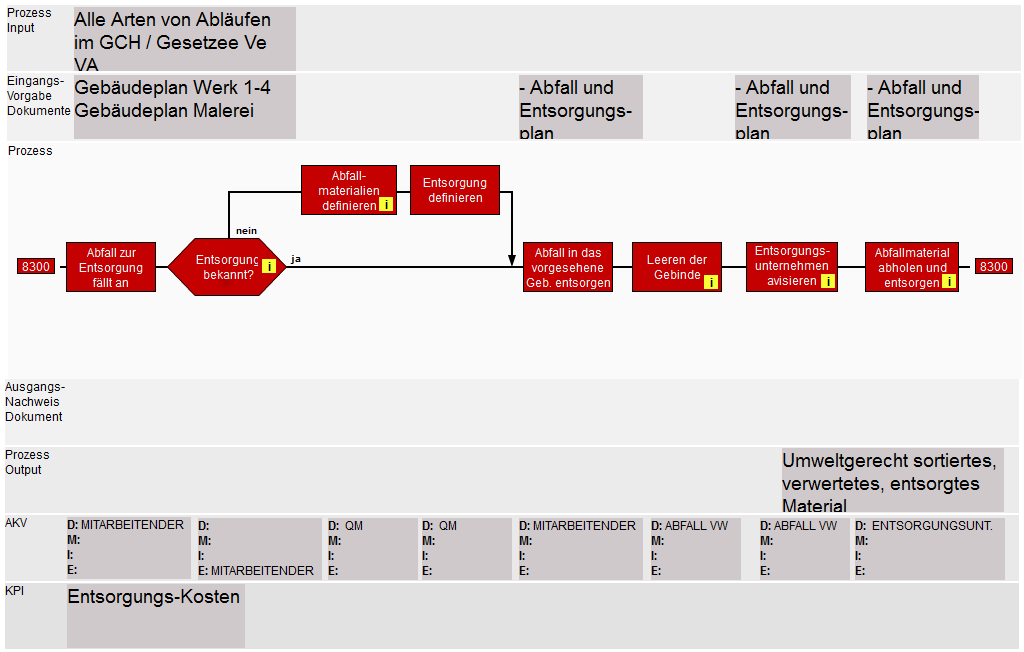
\includegraphics[scale=0.45]{recherche/orgmanager.png}
\newpage

\section{Zukünftige Entwicklungen}
\label{sec:orgd33a30e}
Der Branchenverband gibt an \cite{ref1} dass, das Potential
''kostengünstiger Massnahmen vielerorts bereits abgeschöpft wurde,``
Dies lässt darauf schliessen das man wohl nicht mit allzu viel
Motivation von Seiten der Industrie rechnen kann. Auch der
Branchenverband schreibt im gleichen Satz dass, dadurch die
''Reduktionskurve allmählich abflacht.`` Darunter versteht der Autor
das weitere Verbesserungen Geld kosten würden welches die Industrie
nicht bereit ist zu zahlen.

Je nachdem wie sich die Preise von fossilen Brennstoffen entwickeln
kann sich das noch etwas ändern da dann plötzlich wieder Massnahmen
interessant werden welche momentan noch als zu teuer angesehen
werden. Gerade im Bereich Erdöl werden hier sicherlich noch einige
Änderungen zu sehen sein da dies ja auch für Kunststoffe benötigt wird.
Je nachdem kann sowas aber auch durch neue Fertigungsverfahren
abgefangen werden. Etwa mit 3D Druck, welcher stabilere Strukturen bei
weniger Material ermöglicht.

Von Seiten der Gesetzgeber ist anzunehmen das der Druck, ökologisch zu
handeln, steigen wird. Gerade weil, die Politik in der Schweiz doch
noch sehr volksnah ist und in der Bevölkerung das Bewusstsein für
aktiven Umweltschutz immer weiter zunimmt.  Die Schweiz hätte aufgrund
der vielen Forschungsinstitutionen und der finanziellen Situation
durchaus das Potential eine absolut führende Rolle
einzunehmen. Nichtsdestotrotz braucht man den internationalen
Vergleich bereits jetzt nicht zu scheuen.

Zusammenfassend gibt es sicher einen globalen Trend zu aktivem
Umweltschutz, auch in der Industrie. Wie stark dieser ausgelebt wird
ist aber vor allem eine Kostenfrage.
